\documentclass[12pt,a4paper]{article}

\usepackage[utf8]{inputenc}
\usepackage[T1]{fontenc}
\usepackage{lmodern}
\usepackage{geometry}
\usepackage{array}
\usepackage{booktabs}
\usepackage{longtable}
\usepackage{hyperref}
\usepackage{xcolor}
\usepackage{listings}
\usepackage{amsmath}
\usepackage{tikz}
\usepackage{pgfplots}
\pgfplotsset{compat=1.18}

\geometry{margin=2.5cm}
\hypersetup{
    colorlinks=true,
    linkcolor=blue,
    urlcolor=blue
}

\lstdefinestyle{bashstyle}{
    basicstyle=\ttfamily\small,
    breaklines=true,
    frame=single,
    backgroundcolor=\color{gray!8},
    columns=fullflexible
}

\title{HQC Decoder and CPU/NPU Simulation}
\author{}
\date{}

\begin{document}

\maketitle

\section{What is the decoder in HQC?}

HQC, short for \textit{Hamming Quasi-Cyclic}, is a post-quantum cryptosystem based on error-correcting codes. In HQC, the message is first encoded with a concatenated error-correcting code before encryption. The decoder is the component that recovers the original message from a noisy received codeword.

In this project, the analyzed component is the HQC-128 codec decoder. The main parameters are:

\begin{center}
\begin{tabular}{ll}
\toprule
Parameter & Meaning \\
\midrule
\texttt{PARAM\_K = 16} & Original message length: 16 bytes \\
\texttt{PARAM\_N1 = 46} & Reed--Solomon codeword length: 46 bytes \\
\texttt{PARAM\_N2 = 384} & Each RS byte is encoded into 384 repeated RM bits \\
\texttt{PARAM\_N1N2 = 17664} & Concatenated codeword length: 17664 bits \\
\texttt{PARAM\_DELTA = 15} & Reed--Solomon corrects up to 15 symbol errors \\
\texttt{PARAM\_M = 8} & Finite field: $GF(2^8)$ \\
\bottomrule
\end{tabular}
\end{center}

The concatenated encoder works as follows:

\[
m \xrightarrow{\text{Reed--Solomon encode}} c_{RS}
\xrightarrow{\text{Reed--Muller encode}} c_{RM}.
\]

The decoder performs the inverse operation:

\[
c_{RM}^{'} \xrightarrow{\text{Reed--Muller decode}} \hat{c}_{RS}
\xrightarrow{\text{Reed--Solomon decode}} \hat{m}.
\]

In the source code, this flow corresponds to \texttt{code\_decode}: it first calls \texttt{reed\_muller\_decode}, then calls \texttt{reed\_solomon\_decode}. Therefore, the HQC decoder is not just a single function. It is a two-stage decoding pipeline:

\begin{itemize}
    \item Reed--Muller decode: reduces bit-level noise and recovers the 46-byte intermediate RS codeword.
    \item Reed--Solomon decode: corrects symbol errors over $GF(2^8)$ and recovers the 16-byte message.
\end{itemize}

\section{What is an NPU and what is the HQC decoder algorithm?}

\subsection{What is an NPU?}

NPU stands for \textit{Neural Processing Unit}. It is a specialized processor designed for highly parallel workloads, especially AI workloads such as matrix multiplication, convolution, vector arithmetic, and tensor processing. Compared with a CPU, an NPU usually has more parallel compute units and is more efficient when the workload has regular data layout, many independent operations, and limited complex branching.

In this project, the actual acceleration target is Qualcomm Hexagon with HVX intrinsics. HVX is Hexagon's vector unit, not a narrow neural-network-only NPU. However, the optimization idea is similar to NPU programming: identify highly parallel kernels, move them to vector lanes, and leave complex control flow or irregular logic in scalar CPU/DSP code.

\subsection{HQC decoder algorithm}

The HQC-128 decoder in this project has two main stages.

\subsubsection*{Stage 1: Reed--Muller decode}

Each byte of the Reed--Solomon codeword is encoded with a duplicated Reed--Muller code. For HQC-128, there are 46 Reed--Muller blocks, and each block has 384 bits. The decoder must convert each 384-bit block back into one RS byte.

The main steps are:

\begin{enumerate}
    \item Expand and sum the repeated RM block into signed reliability values.
    \item Run the Hadamard transform to find the most reliable coefficient.
    \item Find the peak, meaning the index with the largest absolute value.
    \item Recover the corresponding RS byte from the peak index and sign.
\end{enumerate}

This stage is suitable for vector/NPU-style acceleration because many lanes can perform addition, subtraction, absolute value, and maximum search in parallel.

\subsubsection*{Stage 2: Reed--Solomon decode}

After Reed--Muller decoding, the decoder obtains 46 RS bytes, but some symbol errors may remain. The Reed--Solomon decoder corrects these errors over $GF(2^8)$.

The main steps are:

\begin{enumerate}
    \item Compute syndromes to detect errors.
    \item Compute the error-locator polynomial, usually called ELP.
    \item Find roots with FFT/additive FFT to locate error positions.
    \item Compute the auxiliary polynomial and error values.
    \item Correct the erroneous bytes and return the 16-byte message.
\end{enumerate}

In the current intrinsic implementation, RS syndrome computation has been vectorized with HVX. For each received RS byte, the implementation computes multiple independent products with syndrome constants across vector lanes. The default path uses a hardware-style fixed-flow $GF(2^8)$ multiplication shape instead of data-dependent table lookup.

\section{How is running on a CPU different from running on an NPU?}

A CPU is a general-purpose processor. It handles control flow, branching, irregular memory access, and normal C code well. When the HQC decoder runs on a CPU or scalar implementation, most Reed--Muller and Reed--Solomon loops are executed sequentially, unless the compiler can automatically use SIMD.

An NPU or vector accelerator is stronger on regular and independent operations. In the HQC decoder, suitable kernels include:

\begin{itemize}
    \item additions and subtractions in the Reed--Muller Hadamard transform;
    \item absolute value and maximum search in RM peak search;
    \item summing repeated blocks in RM expand/sum;
    \item computing many RS syndromes in parallel;
    \item some $GF(2^8)$ multiplications when they can be expressed in a vector-friendly fixed-flow form.
\end{itemize}

The key differences are summarized below:

\begin{center}
\begin{tabular}{p{0.28\linewidth}p{0.32\linewidth}p{0.32\linewidth}}
\toprule
Criterion & CPU/scalar & NPU/vector accelerator \\
\midrule
Main goal & Flexible and easy to program & High throughput for parallel arithmetic \\
Control flow & Handles branches well & Less efficient with irregular branches \\
Data access & Accepts irregular memory access & Best with aligned and regular data layout \\
HQC decoder & Easy to implement the whole RS/RM pipeline & Accelerates kernels such as Hadamard, peak search, and syndrome \\
Main risk & Slower on large loops & Requires correctness and side-channel validation \\
\bottomrule
\end{tabular}
\end{center}

The important point is that the whole HQC decoder does not automatically become faster on an NPU. Parts with many lookup tables, data dependencies, or sequential dependencies, such as some Reed--Solomon ELP and error-value steps, are harder to vectorize. The practical approach is to benchmark each stage, identify the real hot path, and only then move selected kernels to intrinsics or vector code.

\section{How to run the simulation}

\subsection{Simulation data}

The decode benchmark in this repository does not measure encoding. The fixture corpus is generated on the host first, and the benchmark binary measures only decoding. The data set contains:

\begin{itemize}
    \item 16 deterministic fixtures;
    \item each fixture has one random 16-byte message;
    \item each fixture has one corrupted HQC-128 codeword;
    \item the Reed--Solomon symbol error count covers 0 through 15;
    \item each codeword has 17664 bits, or 2208 bytes;
    \item the expected output is the decoded 16-byte message.
\end{itemize}

If \texttt{HQC128\_BENCH\_ITERS=10}, then the total number of decodes is:

\[
10 \times 16 = 160.
\]

\subsection{Simulation commands}

Generate the fixture for the scalar version:

\begin{lstlisting}[style=bashstyle]
cd hqc_lab_scalar
bash scripts/gen_hqc128_decode_fixture.sh
\end{lstlisting}

Run the decode benchmark on the host CPU:

\begin{lstlisting}[style=bashstyle]
bash scripts/run_hqc128_decode_bench_host.sh
\end{lstlisting}

Run the scalar version on the Hexagon simulator:

\begin{lstlisting}[style=bashstyle]
bash scripts/run_hqc128_decode_bench_hexagon.sh
\end{lstlisting}

Run the HVX intrinsic version on the Hexagon simulator:

\begin{lstlisting}[style=bashstyle]
cd ../hqc_lab_insintric
bash scripts/gen_hqc128_decode_fixture.sh
HQC128_BENCH_ITERS=10 bash scripts/run_hqc128_decode_bench_hexagon.sh
\end{lstlisting}

Run the HVX intrinsic version with the experimental GF LUT path:

\begin{lstlisting}[style=bashstyle]
HQC128_BENCH_ITERS=10 HQC_GF_LUT_MUL=1 \
  bash scripts/run_hqc128_decode_bench_hexagon.sh
\end{lstlisting}

Note: the GF LUT path is faster in simulation, but it uses data-dependent table lookup. Therefore, it should not be the default cryptographic implementation if the threat model includes side-channel leakage.

\subsection{Simulation results}

The following numbers come from the repository benchmark using the 16-fixture corpus. The estimated cost per decode is computed as:

\[
\frac{\text{Pcycles}_{10\ \text{iters}} - \text{Pcycles}_{1\ \text{iter}}}{9 \times 16}.
\]

\begin{center}
\begin{tabular}{lrrrr}
\toprule
Variant & Iters & Fixtures & Total Pcycles & Pcycles/decode \\
\midrule
Scalar & 10 & 16 & 155,173,506 & 953,767 \\
Default CT HVX intrinsic & 10 & 16 & 43,082,676 & 252,490 \\
Fastest non-CT HVX intrinsic & 10 & 16 & 12,866,145 & 58,605 \\
\bottomrule
\end{tabular}
\end{center}

\begin{figure}[htbp]
\centering
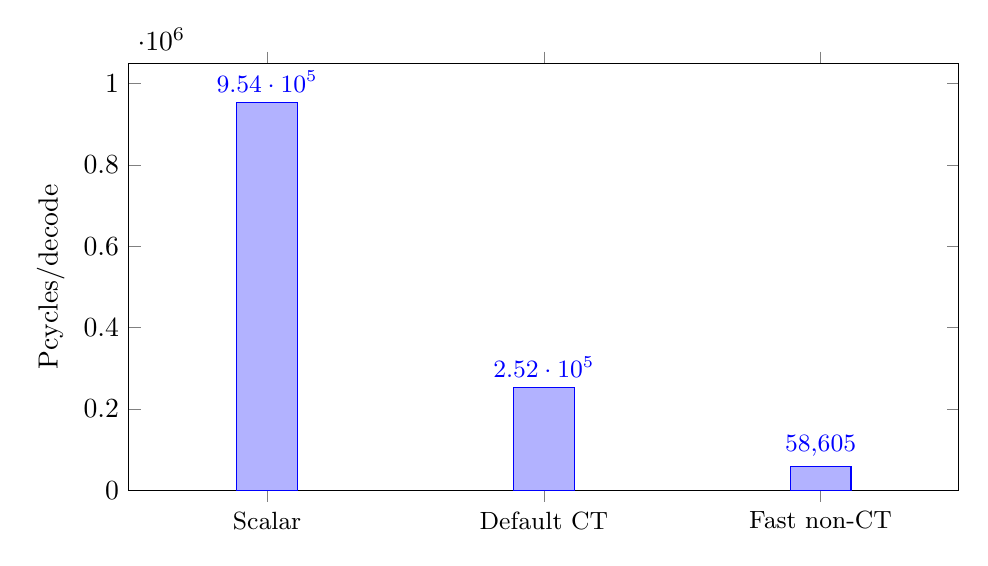
\begin{tikzpicture}
\begin{axis}[
    ybar,
    width=\linewidth,
    height=7cm,
    bar width=22pt,
    ylabel={Pcycles/decode},
    symbolic x coords={Scalar,Default CT,Fast non-CT},
    xtick=data,
    ymin=0,
    enlarge x limits=0.25,
    nodes near coords,
    nodes near coords style={font=\small},
    yticklabel style={/pgf/number format/fixed},
    x tick label style={font=\small},
]
\addplot coordinates {
    (Scalar,953767)
    (Default CT,252490)
    (Fast non-CT,58605)
};
\end{axis}
\end{tikzpicture}
\caption{Hexagon simulator full-decode cost. Lower is better.}
\end{figure}

Compared with the scalar version, the default HVX intrinsic version is faster by approximately:

\[
1 - \frac{252490}{953767} \approx 73.5\%.
\]

The fastest non-CT HVX intrinsic version is faster than scalar by approximately:

\[
1 - \frac{58605}{953767} \approx 93.9\%.
\]

The full benchmark table is:

\begin{center}
\begin{tabular}{lrrrr}
\toprule
Variant & Iters & Fixtures & Total instructions & Total Pcycles \\
\midrule
Scalar & 10 & 16 & 139,903,064 & 155,173,506 \\
Scalar & 1 & 16 & 15,658,494 & 17,831,082 \\
Default CT HVX intrinsic & 10 & 16 & 35,464,291 & 43,082,676 \\
Default CT HVX intrinsic & 1 & 16 & 5,268,713 & 6,724,140 \\
Fastest non-CT HVX intrinsic & 10 & 16 & 9,888,738 & 12,866,145 \\
Fastest non-CT HVX intrinsic & 1 & 16 & 3,370,774 & 4,427,013 \\
\bottomrule
\end{tabular}
\end{center}

\subsection{Substage analysis}

The substage benchmark was measured for all three simulator variants: scalar first, then default CT HVX, then fastest non-CT HVX.  RM substage costs are converted from per-block cost to per-decode cost by multiplying by 46 RM blocks.  RS substage costs are already per decode.

\begin{center}
\begin{tabular}{lrrr}
\toprule
Substage & Scalar & Default CT HVX & Fastest non-CT HVX \\
\midrule
RM expand/sum & 149,742 & 51,624 & 20,988 \\
RM Hadamard & 263,167 & 18,907 & 18,908 \\
RM find peak & 71,216 & 8,012 & 6,080 \\
RS syndrome & 162,309 & 8,637 & 8,637 \\
RS ELP & 119,591 & 81,860 & 7,879 \\
RS roots/FFT & 105,765 & 3,447 & 2,132 \\
RS Z polynomial & 13,044 & 11,146 & 1,141 \\
RS error values & 143,106 & 87,397 & 6,004 \\
RS correction & 439 & 439 & 439 \\
\midrule
Isolated substage sum & 1,028,378 & 271,469 & 72,208 \\
Full decode estimate & 953,767 & 252,490 & 58,605 \\
Substage sum / full decode & 107.8\% & 107.5\% & 123.2\% \\
\bottomrule
\end{tabular}
\end{center}

\begin{figure}[htbp]
\centering
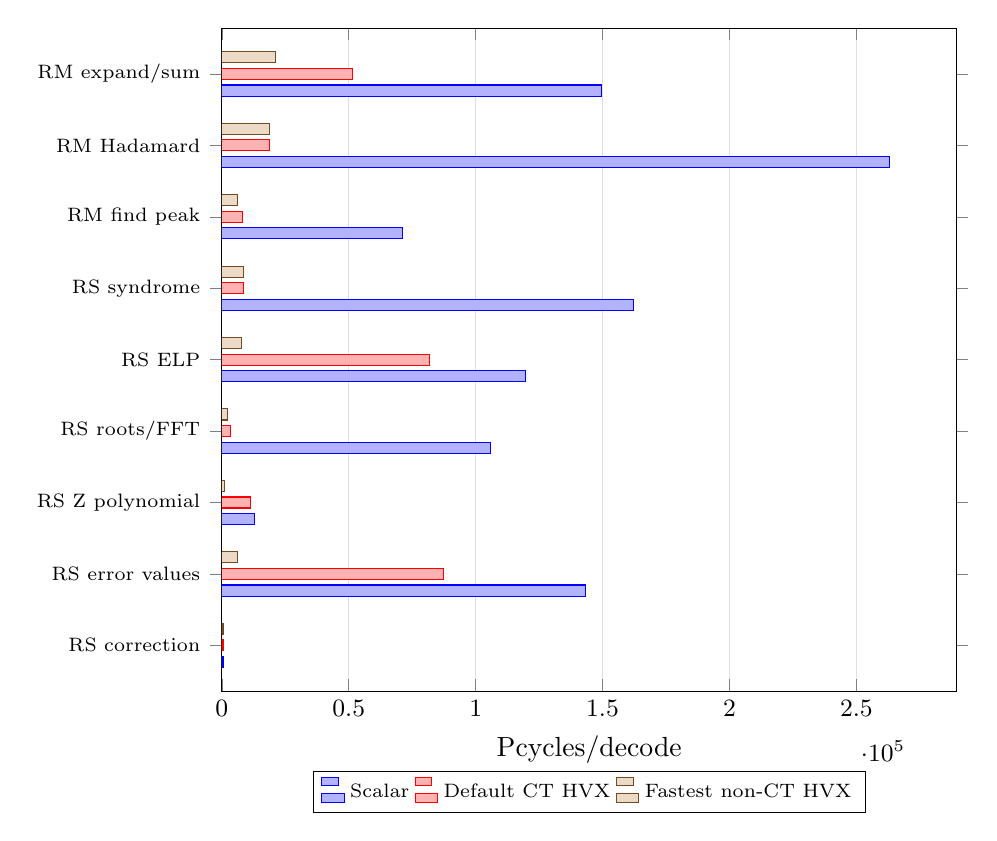
\begin{tikzpicture}
\begin{axis}[
    xbar,
    width=0.9\linewidth,
    height=10cm,
    bar width=4pt,
    xlabel={Pcycles/decode},
    symbolic y coords={RM expand/sum,RM Hadamard,RM find peak,RS syndrome,RS ELP,RS roots/FFT,RS Z polynomial,RS error values,RS correction},
    ytick=data,
    y dir=reverse,
    xmin=0,
    enlarge y limits=0.08,
    legend style={at={(0.5,-0.12)},anchor=north,legend columns=3,font=\scriptsize},
    x tick label style={font=\small},
    yticklabel style={font=\scriptsize},
    xmajorgrids=true,
    grid style={gray!25},
]
\addplot coordinates {
    (149742,RM expand/sum)
    (263167,RM Hadamard)
    (71216,RM find peak)
    (162309,RS syndrome)
    (119591,RS ELP)
    (105765,RS roots/FFT)
    (13044,RS Z polynomial)
    (143106,RS error values)
    (439,RS correction)
};
\addplot coordinates {
    (51624,RM expand/sum)
    (18907,RM Hadamard)
    (8012,RM find peak)
    (8637,RS syndrome)
    (81860,RS ELP)
    (3447,RS roots/FFT)
    (11146,RS Z polynomial)
    (87397,RS error values)
    (439,RS correction)
};
\addplot coordinates {
    (20988,RM expand/sum)
    (18908,RM Hadamard)
    (6080,RM find peak)
    (8637,RS syndrome)
    (7879,RS ELP)
    (2132,RS roots/FFT)
    (1141,RS Z polynomial)
    (6004,RS error values)
    (439,RS correction)
};
\legend{Scalar,Default CT HVX,Fastest non-CT HVX}
\end{axis}
\end{tikzpicture}
\caption{Grouped simulator substage costs.  Each substage shows scalar first, then default CT HVX, then fastest non-CT HVX.  Lower is better.}
\end{figure}

The scalar breakdown shows that RM Hadamard, RS syndrome, RM expand/sum, and RS error values are all large contributors before HVX optimization.  In the default CT HVX path, the dominant remaining costs are RS error values, RS ELP, and RM expand/sum.  The fastest non-CT path reduces RS algebra costs sharply, but it remains benchmark-only because it uses side-channel-relaxed control flow and data-dependent lookup tables.

\section{Real-device board results}

The real-device measurements use the same 16-fixture decode corpus, but the metric is host-observed wall-clock latency rather than simulator Pcycles. Each main board run uses \texttt{iters=10000}, corresponding to 160,000 total decodes per variant.

\begin{center}
\begin{tabular}{llrrr}
\toprule
Board & Variant & us/decode & Throughput & Speedup vs CPU \\
\midrule
RB3 Gen 2 & CPU scalar & 106.479 & 9,391.5 & 1.00x \\
RB3 Gen 2 & cDSP scalar FastRPC & 484.554 & 2,063.8 & 0.22x \\
RB3 Gen 2 & cDSP default CT HVX & 110.908 & 9,016.5 & 0.96x \\
RB3 Gen 2 & cDSP fastest non-CT HVX & 47.495 & 21,054.8 & 2.24x \\
QRD8650 & CPU scalar & 70.971 & 14,090.3 & 1.00x \\
QRD8650 & cDSP scalar FastRPC & 369.007 & 2,710.0 & 0.19x \\
QRD8650 & cDSP default CT HVX & 86.633 & 11,542.9 & 0.82x \\
QRD8650 & cDSP fastest non-CT HVX & 37.456 & 26,698.0 & 1.89x \\
\bottomrule
\end{tabular}
\end{center}

\begin{figure}[htbp]
\centering
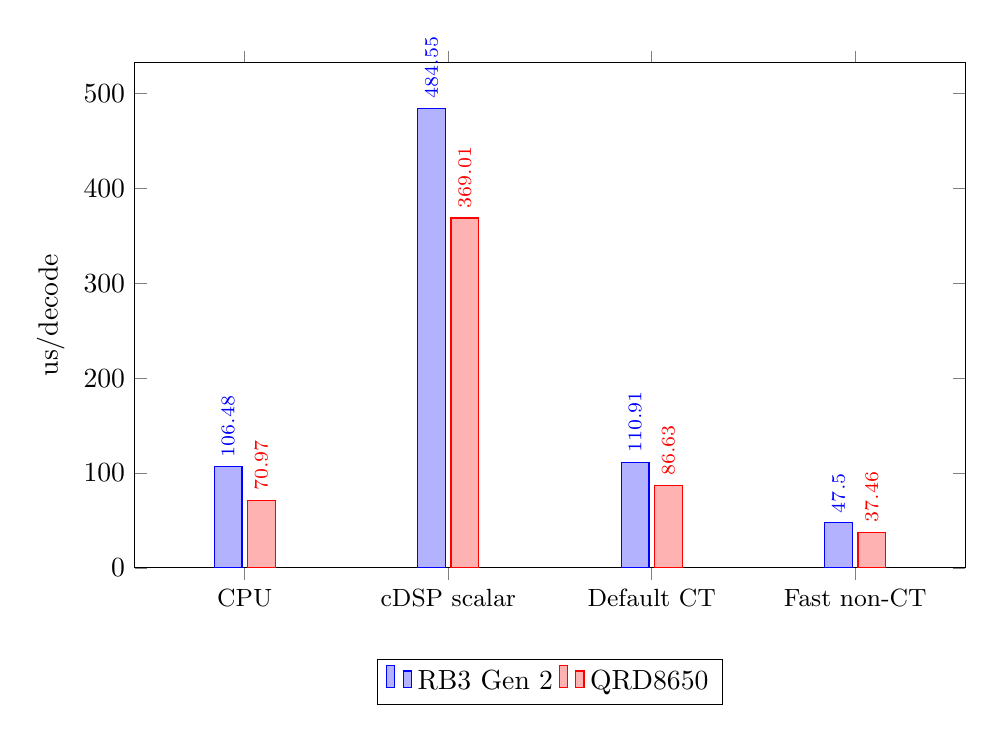
\begin{tikzpicture}
\begin{axis}[
    ybar,
    width=\linewidth,
    height=8cm,
    bar width=10pt,
    ylabel={us/decode},
    symbolic x coords={CPU,cDSP scalar,Default CT,Fast non-CT},
    xtick=data,
    ymin=0,
    enlarge x limits=0.18,
    legend style={at={(0.5,-0.18)},anchor=north,legend columns=2},
    nodes near coords,
    nodes near coords style={font=\scriptsize,rotate=90,anchor=west},
    yticklabel style={/pgf/number format/fixed},
    x tick label style={font=\small},
]
\addplot coordinates {
    (CPU,106.479)
    (cDSP scalar,484.554)
    (Default CT,110.908)
    (Fast non-CT,47.495)
};
\addplot coordinates {
    (CPU,70.971)
    (cDSP scalar,369.007)
    (Default CT,86.633)
    (Fast non-CT,37.456)
};
\legend{RB3 Gen 2,QRD8650}
\end{axis}
\end{tikzpicture}
\caption{Real-device decode latency. Lower is better.}
\end{figure}

On both real devices, cDSP scalar through FastRPC is slower than the ARM64 CPU scalar baseline. The default CT HVX path recovers most of that gap but is still slightly slower than CPU scalar on these wall-clock measurements. The fastest non-CT path is the best measured real-device variant, but it remains benchmark-only because it uses side-channel-relaxed RS control flow and data-dependent lookup tables.

\section{Completed work in this project}

This repository already contains both a portable scalar baseline and an optimized Hexagon/HVX intrinsic version for HQC-128 decode experiments. The work completed so far can be summarized as follows.

\subsection{Scalar baseline}

The scalar baseline was separated into \texttt{hqc\_lab\_scalar}. It keeps the reference HQC-128 concatenated codec structure:

\begin{itemize}
    \item \texttt{code.c}: concatenated codec wrapper;
    \item Reed--Solomon encode/decode;
    \item duplicated Reed--Muller encode/decode;
    \item finite-field arithmetic over $GF(2^8)$;
    \item FFT support used by Reed--Solomon decode.
\end{itemize}

The scalar Hexagon benchmark intentionally builds without \texttt{-mhvx}. This gives a fair baseline for measuring the benefit of HVX/vector acceleration.

\subsection{HVX intrinsic implementation}

The optimized version was placed in \texttt{hqc\_lab\_insintric}. The main completed optimization passes are:

\begin{enumerate}
    \item Vectorized the Reed--Muller Hadamard transform with HVX halfword add/sub operations.
    \item Vectorized RM peak search using HVX absolute value, maximum reduction, equality predicates, and index selection.
    \item Removed scalar even/odd gather in the Hadamard path by using HVX deal/deinterleave operations.
    \item Partially vectorized RM expand/sum: bit extraction is still scalar, but repeated-block summation uses HVX halfword operations.
    \item Added a hardware-style fixed-flow $GF(2^8)$ multiplier based on the Verilog hardware design shape.
    \item Vectorized Reed--Solomon syndrome computation by computing multiple independent GF products across HVX lanes.
    \item Added an optional GF LUT multiplication path for performance experiments, while keeping it disabled by default because of side-channel concerns.
\end{enumerate}

Disassembly confirmed that the intrinsic binary contains HVX instructions such as \texttt{vmem}, \texttt{vadd}, \texttt{vsub}, \texttt{vabs}, \texttt{vmax}, \texttt{vror}, and \texttt{vdeal}.

\subsection{Benchmark and validation infrastructure}

The benchmark setup was also extended:

\begin{itemize}
    \item A deterministic 16-fixture decode corpus was generated.
    \item The corpus covers RS symbol error counts from 0 to 15.
    \item The benchmark measures decode only, so encode is not included in the timed binary.
    \item Host, scalar Hexagon, and HVX Hexagon benchmark scripts were added.
    \item Stage-level benchmarking was added to split Reed--Muller and Reed--Solomon costs.
    \item Substage-level benchmarking was added to identify the remaining hot spots inside RM and RS decode.
\end{itemize}

All reported benchmark variants pass correctness validation against the expected 16-byte messages in the fixture corpus.

\subsection{Current result}

The current default CT intrinsic path uses HVX-assisted Reed--Muller kernels, hardware-style GF multiplication, fused RM operations, and HVX RS root support. On the 16-fixture corpus, the estimated simulator decode cost improved from 953,767 Pcycles/decode for scalar to 252,490 Pcycles/decode for the default CT intrinsic implementation. This is about a 73.5\% reduction in estimated Pcycles per decode.

The fastest non-CT experiment further reduces the estimate to 58,605 Pcycles/decode, about 93.9\% lower than scalar. However, it remains a benchmark-only option because side-channel-relaxed control flow and data-dependent lookup are not automatically acceptable for cryptographic code.

The most useful result of the substage benchmark is that the next optimization targets are now clear. RM Hadamard, RM peak search, and RS syndrome are no longer dominant. The remaining high-cost areas are RS error values, RS ELP, and RM expand/sum.

\section{Conclusion}

The HQC decoder is a concatenated decoder consisting of Reed--Muller decode followed by Reed--Solomon decode. Reed--Muller handles bit-level noise and recovers the RS codeword, while Reed--Solomon corrects symbol errors and recovers the 16-byte message.

A CPU is suitable for running the full algorithm flexibly, but an NPU or vector accelerator is better for highly parallel kernels. In this project's simulation, the scalar version costs about 953,767 Pcycles/decode, while the default CT HVX intrinsic version costs about 252,490 Pcycles/decode, which is about 73.5\% lower. The fastest non-CT version reaches about 58,605 Pcycles/decode, but it requires side-channel consideration because it uses relaxed control flow and data-dependent lookup.

\end{document}
